% !TEX root = ../../../I4PRJ, Grp3 - Rapport.tex
\subsubsection{Konceptuel Design}
Det konceptuelle design udarbejdes ved analyse og diskussion af user stories, som eksempel er user story omhandlende login behandlet og kan ses på figuren nedenfor:

\begin{figure}
	\centering
	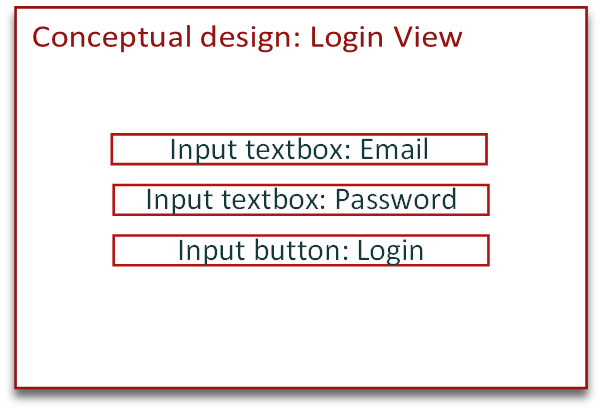
\includegraphics[width=0.5\linewidth]{figs/design/concuptuel_design_loginview}
	\caption{Konceptuelt design af LoginView}
	\label{fig:conceptualdesignview}
\end{figure}

De konceptuelle design udvides til et grafisk design.

\subsubsection{Grafisk Design}
\begin{figure}
	\centering
	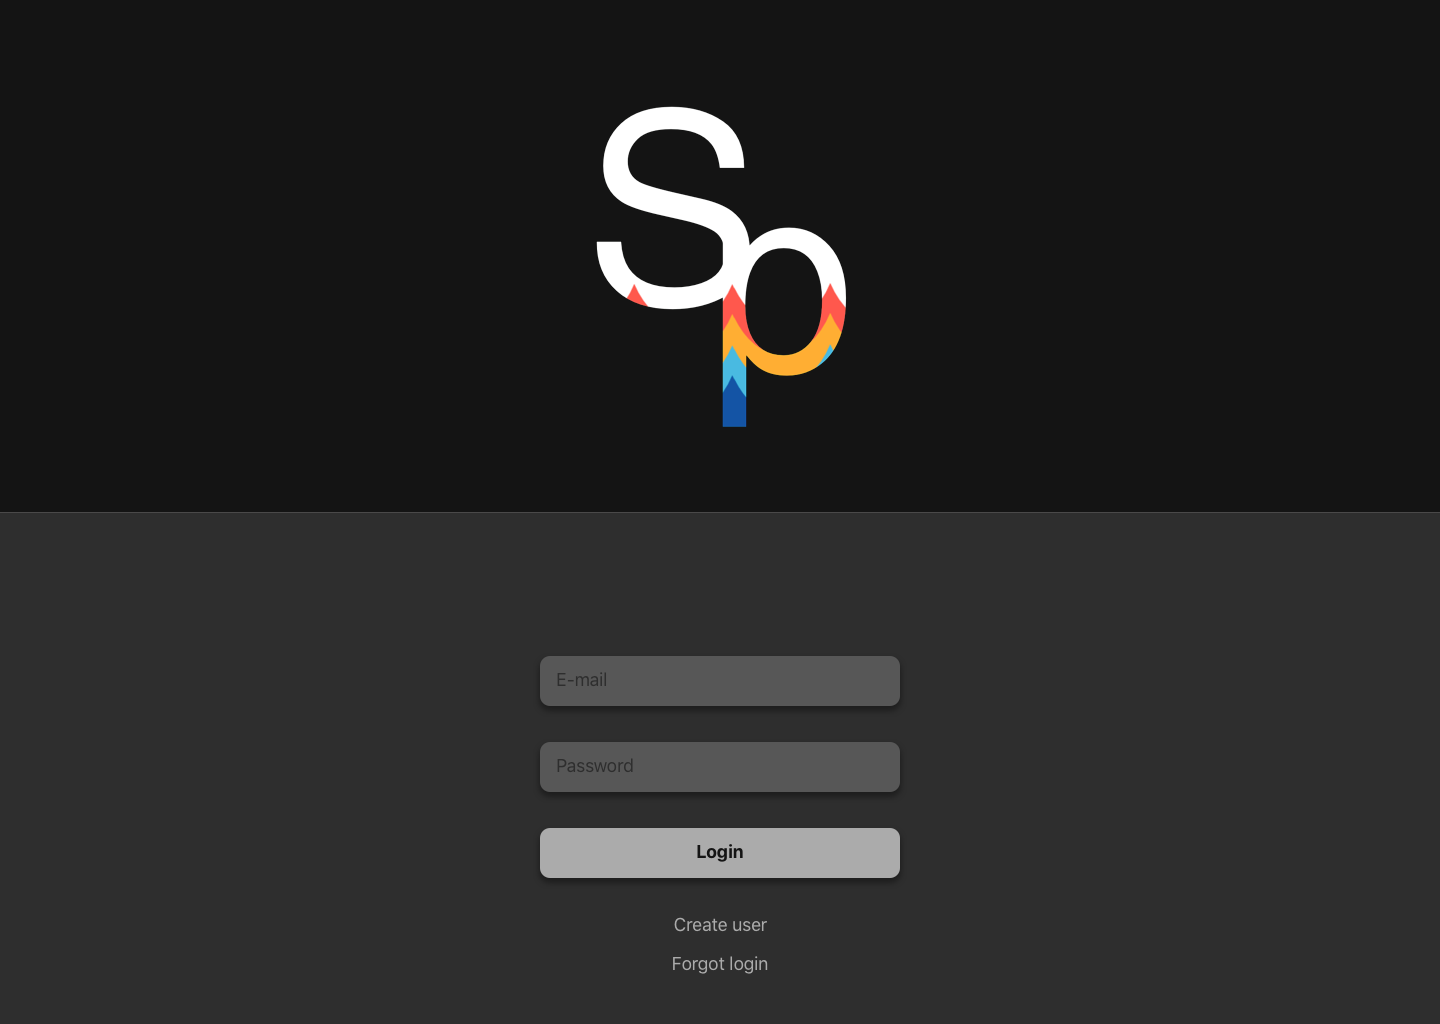
\includegraphics[width=0.5\linewidth]{figs/design/DesktopHDLogin}
	\caption{Grafisk design af LoginView}
	\label{fig:graphicaldesign}
\end{figure}

Udviklere af views til de forskellige applikationer stræber efter at opnå et visuelt design, der ligner dette mest muligt.